\documentclass[12pt, a4paper]{report}
\usepackage[utf8]{inputenc}
\usepackage[english, russian]{babel}

\usepackage{graphicx}
\usepackage{listings}
\usepackage{color}

\usepackage{amsmath}
\usepackage{pgfplots}
\usepackage{url}
\usepackage{flowchart}
\usepackage{tikz}
\DeclareGraphicsExtensions{.pdf,.png,.jpg,.svg}
\usetikzlibrary{shapes, arrows}

\usepackage{pgfplotstable}

\renewcommand\contentsname{Содержание}

\usepackage{geometry}
\geometry{left=3cm}
\geometry{right=1cm}
\geometry{top=2cm}
\geometry{bottom=2cm}

\lstset{ %
language=C++,                 % выбор языка для подсветки (здесь это С)
basicstyle=\small\sffamily, % размер и начертание шрифта для подсветки кода
numbers=left,               % где поставить нумерацию строк (слева\справа)
numberstyle=\tiny,           % размер шрифта для номеров строк
stepnumber=1,                   % размер шага между двумя номерами строк
numbersep=-5pt,                % как далеко отстоят номера строк от         подсвечиваемого кода
backgroundcolor=\color{white}, % цвет фона подсветки - используем         \usepackage{color}
showspaces=false,            % показывать или нет пробелы специальными     отступами
showstringspaces=false,      % показывать или нет пробелы в строках
showtabs=false,             % показывать или нет табуляцию в строках
frame=single,              % рисовать рамку вокруг кода
tabsize=2,                 % размер табуляции по умолчанию равен 2 пробелам
captionpos=t,              % позиция заголовка вверху [t] или внизу [b] 
breaklines=true,           % автоматически переносить строки (да\нет)
breakatwhitespace=false, % переносить строки только если есть пробел
escapeinside={\%*}{*)},   % если нужно добавить комментарии в коде
keywordstyle=\color{blue}\ttfamily,
stringstyle=\color{red}\ttfamily,
commentstyle=\color{green}\ttfamily,
morecomment=[l][\color{magenta}]{\#},
columns=fullflexible }

\usepackage{titlesec}
\titleformat{\chapter}[hang]{\LARGE\bfseries}{\thechapter{.} }{0pt}{\LARGE\bfseries}
\titleformat*{\section}{\Large\bfseries}
\titleformat*{\subsection}{\large\bfseries}

\begin{document}

    \begin{titlepage}

        \begin{center}
            \Large
            {\sl Государственное образовательное учреждение высшего профессионального образования\\
            {\bf«Московский государственный технический университет имени Н.Э. Баумана»\\
				(МГТУ им. Н.Э. Баумана)}}
				\noindent\rule{\textwidth}{2pt}
            \vspace{3cm}

			{\scshape\LARGE Рубежный контроль №2 \par}
			\vspace{0.5cm}	
			{\scshape\LARGE по курсу «Анализ алгоритмов» \par}
			\vspace{1.5cm}
			{\huge\bfseries Конечные автоматы и регулярные выражения \par}
			\vspace{2cm}
			\Large Выполнил: Сорокин А.П., гр. ИУ7-52Б\\
			\vspace{0.5cm}
			{\Large Преподаватели: Волкова Л.Л., Строганов Ю.В.}
		
			\vfill
			\Large \textit {Москва, 2019 г.}
            
        \end{center}

    \end{titlepage}
	
	\tableofcontents

	\chapter*{Введение}
	\addcontentsline{toc}{chapter}{Введение}
	\hspace{0.5cm}Цель рубежного контроля: при помощи конечного автомата и регулярного выражения
	написать программу для поиска критических секций в коде.

    \chapter{Аналитическая часть}
	\hspace{0.5cm}В данном разделе будут описаны конечные автоматы и регулярные выражения.
	
	\section{Конечные автоматы}
	\hspace{0.5cm}Конечный автомат — это модель вычислений, основанная на гипотетической машине состояний. В один момент времени только одно состояние может быть активным. Следовательно, для выполнения каких-либо действий машина должна менять свое состояние. Конечные автоматы обычно используются для организации и представления потока выполнения чего-либо ~\cite{ka}.
	
	Конечный автомат можно представить в виде графа, вершины которого являются состояниями, а ребра — переходы между ними. Каждое ребро имеет метку, информирующую о том, когда должен произойти переход.

	\section{Регулярные выражения}
	\hspace{0.5cm}Регулярные выражения — это формальный язык поиска подстроки или подстрок в тексте. Для поиска используется строка-образец (паттерн, или шаблон), состоящая из символов и метасимволов (специальные символы, которые обозначают набор символов).
	
	Это довольно мощный инструмент, который может пригодиться во многих случая —
	поиск, проверка на корректность строки и т.д. Спектр его возможностей трудно уместить
	в одну статью ~\cite{regexp}.
	
	\chapter{Конструкторская часть}
	\hspace{0.5cm}В данном разделе будет построены конечный автомат и регулярное выражение для решения поставленной задачи.
	Шаблон критической секции представлен в листинге \ref{code-crit}.
	\begin{lstlisting}[label=code-crit,caption=Шаблон критической секции]
	::EnterCriticalSection(&obj);
	// ...
	::LeaveCriticalSection(&obj);
	\end{lstlisting}
	
	\section{Конечный автомат}
	\begin{figure}[ht!]
		\centering
		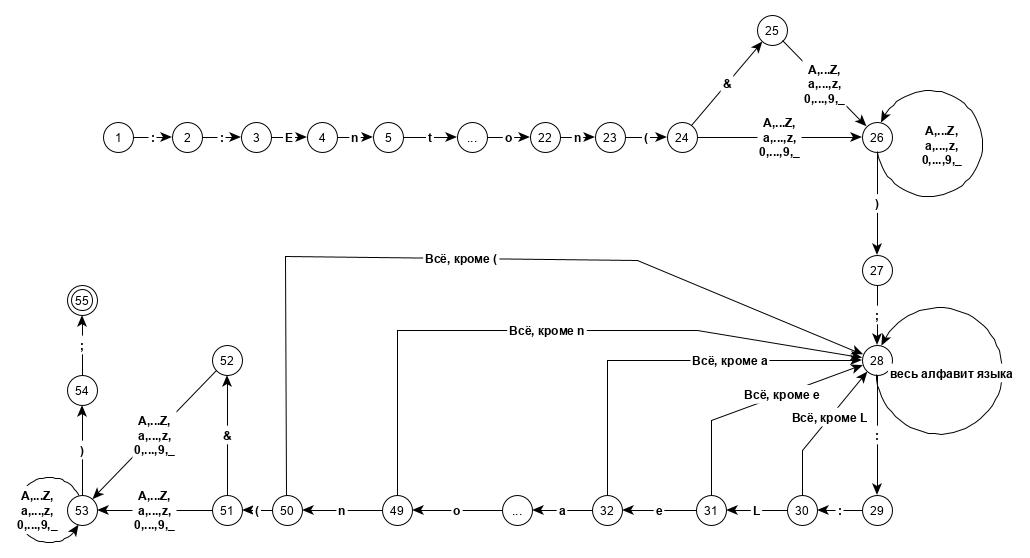
\includegraphics[width=1\linewidth]{ka.jpg}
		\caption{Конечный автомат}
		\label{ris:ka}
	\end{figure}

	\section{Регулярное выражение}
	$::EnterCriticalSection'(' (\&|\lambda) (A+...+Z+a+...+z)^{+} ')';(...)^*
	::LeaveCriticalSection'(' (\&|\lambda) (A+...+Z+a+...+z)^{+} ')';$

	\chapter{Технологическая часть}
	\section{Средства реализации}
	\hspace{0.5cm}Для реализации программы был использован язык Python ~\cite{py} (версия интерпретатора 3.7). Для измерения времени была взята функция time.time() из
	библиотеки time. Данный язык обусловлен тем, что функции, необходимые для реализации регулярного выражения, находятся в встроенной библиотеке re.
	
	\section{Реализации алгоритмов}
	На листингах \ref{code-ka} и \ref{code-regexp} представлены коды реализации поиска критических секций с помощью конечных автоматов и с помощью регулярного выражения.
	
	\lstset{ %
		language=Python,                 % выбор языка для подсветки
		basicstyle=\small\sffamily, % размер и начертание шрифта для подсветки кода
		numbers=left,               % где поставить нумерацию строк (слева\справа)
		numberstyle=\tiny,           % размер шрифта для номеров строк
		stepnumber=1,                   % размер шага между двумя номерами строк
		numbersep=-5pt,                % как далеко отстоят номера строк от         подсвечиваемого кода
		backgroundcolor=\color{white}, % цвет фона подсветки - используем         \usepackage{color}
		showspaces=false,            % показывать или нет пробелы специальными     отступами
		showstringspaces=false,      % показывать или нет пробелы в строках
		showtabs=false,             % показывать или нет табуляцию в строках
		frame=single,              % рисовать рамку вокруг кода
		tabsize=2,                 % размер табуляции по умолчанию равен 2 пробелам
		captionpos=t,              % позиция заголовка вверху [t] или внизу [b] 
		breaklines=true,           % автоматически переносить строки (да\нет)
		breakatwhitespace=false, % переносить строки только если есть пробел
		escapeinside={\%*}{*)},   % если нужно добавить комментарии в коде
		keywordstyle=\color{blue}\ttfamily,
		stringstyle=\color{red}\ttfamily,
		commentstyle=\color{green}\ttfamily,
		morecomment=[l][\color{magenta}]{\#},
		columns=fullflexible }
	
	\begin{lstlisting}[label=code-ka,caption=Поиск с помощью конечного автомата]
	enter_str = "::EnterCriticalSection"
	leave_str = "::LeaveCriticalSection"
	
	name_symbols = "ABCDEFGHIJKLMNOPQRSTUVWXYZabcdefghijklmnopqrstuvxyz_"
	digits = "0123456789"
	
	
	def find_crit(s):
		state = 1
		crit_section = ""
		result = []
	
	for value in s:
		if state == 1:
			if value == ':':
				state = 2
		elif 2 <= state <= 22:
			if value == enter_str[state - 1]:
				state += 1
			else:
				state = 1
		elif state == 23:
			if value == '(':
				state = 24
			else:
				state = 1
		elif state == 24:
			if value == '&':
				state = 25
			elif value in name_symbols:
				state = 26
			else:
				state = 1
		elif state == 25:
			if value in name_symbols + digits:
				state = 26
			else:
				state = 1
		elif state == 26:
			if value in name_symbols + digits:
				state = 26
			elif value == ')':
				state = 27
			else:
				state = 1
		elif state == 27:
			if value == ';':
				state = 28
			else:
				state = 1
	
		elif state == 28:
			if value == ':':
				state = 29

		elif 29 <= state <= 49:
			if value == leave_str[state - 28]:
				state += 1
			else:
				state = 28
		elif state == 50:
			if value == '(':
				state = 51
			else:
				state = 28
		elif state == 51:
			if value == '&':
				state = 52
			elif value in name_symbols:
				state = 53
			else:
				state = 28
		elif state == 52:
			if value in name_symbols + digits:
				state = 53
			else:
				state = 28
		elif state == 53:
			if value in name_symbols + digits:
				state = 53
			elif value == ')':
				state = 54
			else:
				state = 28
		elif state == 54:
			if value == ';':
				state = 55
		else:
			state = 28
	
		if state == 1:
			crit_section = ""
		else:
			crit_section += value
	
		if state == 55:
			result.append(crit_section)
			crit_section = ""
			state = 1
	
	return result
	\end{lstlisting}

	\begin{lstlisting}[label=code-regexp,caption=Поиск с помощью регулярного выражения]
	regexp = r'::EnterCriticalSection\(([A-Za-z&]\w*)\);' +\
		r'((?!::EnterCriticalSection\(\1\);)[\s\S])*' +\
		r'::LeaveCriticalSection\(\1\);'
	
	def find_crit(text):
		tmp = text
	
		found = False
		match = ""
	
		while match is not None:
			match = re.search(regexp, tmp)
			if match is not None:
				found = True
				print(match[0])
				tmp = tmp[match.end():]
				print("############")
	
		if not found:
			print("None")
	\end{lstlisting}

	\newpage


	\chapter{Экспериментальная часть}
	\section{Примеры работы}
	\hspace{0.5cm}На рисунке \ref{fig:example} представлен пример работы программы.
	\begin{figure}[ht!]
		\centering
		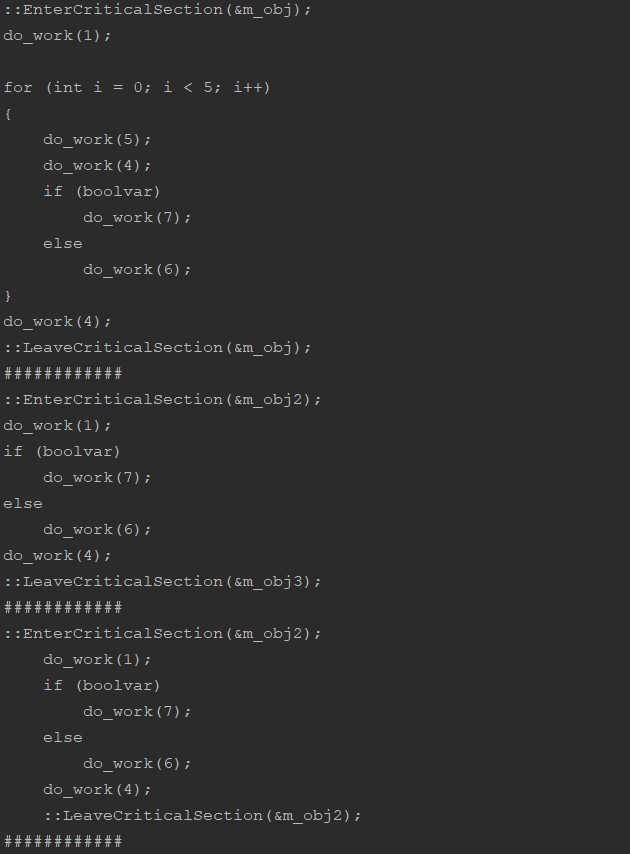
\includegraphics[width=0.7\linewidth]{example.jpg}
		\caption{Пример работы программы}
		\label{fig:example}
	\end{figure}

	\section{Сравнительный анализ}
	В таблице \ref{tab:res} представлены результаты 20 измерений времени в секундах.
	\begin{table}[ht!]
		\caption{Сравнение работы поиска с помощью конченых автоматов и регулярных выражений}
		\label{tab:res}
		\begin{center}
			\pgfplotstabletypeset[
			col sep=semicolon,
			string type,
			columns/KA/.style={column name=Конечный автомат, column type={|c}},
			columns/RegExp/.style={column name=Регулярные выражения, column type={|c|}},
			every head row/.style={before row=\hline,after row=\hline},
			every last row/.style={after row=\hline},
			]{time.csv}
		\end{center}
	\end{table}

	\section{Вывод}
	В среднем поиск с помощью регулярных выражений выполняется в 5 раз дольше, чем поиск с помощью конечного автомата.

	\chapter*{Заключение}
	\addcontentsline{toc}{chapter}{Заключение}
	\hspace{0.5cm}В ходе выполнения рубежного контроля были реализованы программы поиска критических секций в коде с помощью конечного автомата и регулярного выражения. В результате сравнения было выяснено, что алгоритм поиска с помощью регулярных выражений работает дольше, чем алгоритм поиска с помощью конечного автомата.
	
	\newpage
	
	\begin{thebibliography}{}
	\bibitem{ka} Конечные автоматы (finite-state machine) [Электронный ресурс]. https://habr.com/ru/post/358304/
	\bibitem{regexp} Регулярные выражения [Электронный ресурс].  https://habr.com/ru/company/badoo/blog/343310/
	\bibitem{py} Python [Электронный ресурс]. https://www.python.org/
	\end{thebibliography}
	\addcontentsline{toc}{chapter}{Литература}

\end{document}
